\documentclass[10pt,a4paper,twocolumn]{article}
\usepackage[utf8]{inputenc}
\usepackage[english]{babel}
\usepackage[title]{appendix}
\usepackage{graphicx}
\usepackage{amsmath}
\usepackage{amsfonts}
\usepackage{amssymb}
\usepackage{listings}
\usepackage{alltt}
\usepackage{tikz}
\usepackage{graphicx}
\usepackage{hyperref} 

% Configure listings package
\lstset{
    basicstyle=\ttfamily\small,
    breaklines=true,
    frame=single,
    numbers=left,
    numberstyle=\tiny,
    numbersep=5pt,
    showstringspaces=false,
    keywordstyle=\color{blue},
    commentstyle=\color{green!60!black},
    stringstyle=\color{red},
    backgroundcolor=\color{gray!10}
}



\newcommand{\keywords}[1]{\textbf{#1}}

\def\x{{\mathbf x}}
\def\L{{\cal L}}

\title{Memento: A Meta-Cognitive Framework for Self-Evolving System Prompts in AI Systems}
\author{Jaroslaw Nowosad\\
	  \normalsize  SNI Lab, Ireland Research Centre, Huawei \\
	\normalsize e-mail: jaroslaw.nowosad@huawei.com
}


\begin{document}



\twocolumn[
  \begin{@twocolumnfalse}

    \maketitle
    \begin{abstract}


This paper introduces \textit{Memento}, a novel meta-cognitive framework that enables large language models (LLMs) to improve their problem-solving capabilities through self-evolving system prompts autonomously. Memento incorporates meta-cognitive strategies, such as reflection, principle extraction, and knowledge integration, to continuously enhance its reasoning performance across diverse domains. Drawing from and extending recent research on prompt optimization, self-refining models, and autonomous learning systems, Memento demonstrates superior adaptability, accuracy, and generalization. We benchmark its effectiveness across tasks in software engineering, mathematics, and creative writing, and compare it to existing approaches such as PromptBreeder, Auto-Evolve, and Self-Evolving GPT. \newline
The key innovation lies in our structured metacognitive reflection process that extracts, organizes, and applies domain-agnostic reasoning principles through a five-phase learning cycle. Our approach addresses fundamental limitations in current prompt optimization methods by embedding continuous learning directly into the reasoning architecture rather than treating prompts as static optimization targets. \newline

Source code: https://github.com/yarenty/prompt\_learning \newline

\keywords{Keywords: Large Language Models, Meta-Cognitive Learning, Self-Evolving Systems, Prompt Engineering, Cross-Domain Transfer, Autonomous Learning}\newline

    \end{abstract}
    \end{@twocolumnfalse}
]

\newpage


\let\thefootnote\relax\footnotetext{\hspace*{-5mm}

\begin{itemize}
    \item \textbf{Meta-cognitive learning}: AI learns to improve its reasoning strategies.
    \item \textbf{Self-evolving prompts}: The system prompts are updated based on reflection and outcome evaluation.
    \item \textbf{Cross-domain adaptability}: Framework applied across programming, mathematics, and writing.
    \item \textbf{Structured knowledge integration}: Extracts, organizes, and reuses problem-solving principles.
\end{itemize}
}



\newpage
\section{INTRODUCTION}


Current large-language models demonstrate remarkable problem-solving capabilities across diverse domains, yet their performance heavily depends on carefully crafted prompts that remain static throughout interaction. Consider a software engineer debugging a complex algorithm: they do not approach each new bug with the same rigid methodology, but rather adapt their debugging strategies based on lessons learned from previous encounters. Similarly, a mathematician solving proofs develops increasingly sophisticated heuristics that are transferred across problem types. Human experts naturally evolve their problem-solving approaches through reflection and principle extraction—capabilities that current AI systems lack.

This limitation manifests itself in several critical ways:


\begin{itemize}
    \item \textit{Static Knowledge Application}: Traditional prompt engineering treats system instructions as fixed templates, missing opportunities to learn from successful problem-solving patterns. For example, when an LLM successfully debugs a recursive algorithm by first mapping the call stack, this valuable strategy is not retained for future debugging tasks.
    \item \textit{Domain Isolation}: Current approaches do not take advantage of cross-domain insights. A breakthrough in mathematical proof construction (such as working backwards from the desired conclusion) could significantly improve code verification tasks, yet existing systems do not capture or transfer such insights.
    \item \textit{Missed Learning Opportunities}: Every interaction contains valuable metacognitive information about which reasoning approaches work best for specific problem types. Current systems discard this information after each session, repeatedly "re-discovering" effective strategies.
\end{itemize}


\subsection{Theoretical Foundation}

Memento is grounded in three complementary theoretical frameworks:

\begin{itemize}
    \item \textit{Meta-Cognitive Theory}: Building on Flavell's seminal work on metacognition, we implement computational analogues of self-monitoring, self-evaluation, and strategy selection. Our framework operationalizes the "thinking about thinking" process through structured reflection phases that analyze not just what was solved, but how it was solved and why certain approaches succeeded or failed.

\item \textit{Transfer Learning Theory}: We extend classical transfer learning beyond parameter sharing to principle-level knowledge transfer. Unlike traditional approaches that transfer statistical patterns, Memento extracts and transfers abstract reasoning strategies that remain effective across domain boundaries.

\item \textit{Autonomous Learning Systems}: Our approach implements key principles from autonomous learning theory, particularly the concept of intrinsic motivation for improvement and self-directed knowledge acquisition. The system is driven by internal evaluation metrics rather than external rewards, creating a sustainable learning loop.
\end{itemize}

\subsection{Differentiation from Existing Approaches}

Current self-improving systems fall into three categories, each with fundamental limitations that Memento addresses:

\begin{itemize}
    \item \textit{Evolutionary Prompt Optimization (e.g., PromptBreeder[1])}:
    \begin{itemize}
\item \textit{Limitation}: Treats prompts as black-box optimization targets, evolving surface-level wording without understanding underlying reasoning principles.
\item \textit{Memento's Advance}: Extracts and evolves explicit reasoning principles that can be understood, verified, and deliberately applied.
\end{itemize}

    \item \textit{Experience Integration Systems (e.g., Self-Evolving GPT[3])}:
        \begin{itemize}
\item \textit{Limitation}: Accumulates raw experience without structured principle extraction, leading to information overload and inconsistent application.

\item \textit{Memento's Advance}: Implements hierarchical principle organization with confidence scoring and domain-specific indexing for efficient retrieval and application.
\end{itemize}

\item \textit{Self-Reasoning Frameworks (e.g., Auto-Evolve[6])}:
\begin{itemize}
\item \textit{Limitation}: Focuses primarily on error correction rather than principle learning, missing opportunities to extract positive reasoning patterns.
\item \textit{Memento's Advance}: Balances learning from both successes and failures, extracting transferable insights from all problem-solving attempts.
\end{itemize}

\end{itemize}
\subsection{Technical Innovation}

Memento introduces several novel technical contributions:

\begin{itemize}
\item \textit{Hierarchical Principle Architecture}: Unlike flat knowledge stores, our system organizes principles in a multi-level hierarchy that captures both domain-specific techniques and abstract reasoning patterns. This enables efficient retrieval complexity) and natural knowledge organization.

\item \textit{Cross-Domain Transfer Mechanisms}: We implement explicit transfer functions that identify when principles learned in one domain can enhance performance in another. 

\item \textit{Meta-Cognitive Reflection Process}: Our five-phase learning cycle implements computational analogues of expert problem-solving reflection, systematically analyzing strategy effectiveness and extracting reusable insights.
\end{itemize}

\subsection{Concrete Impact Examples}

To illustrate Memento's practical value, consider these real scenarios from our evaluation:

\begin{itemize}
\item \textit{Software Engineering Example}: After successfully debugging several off-by-one errors by carefully tracing array indices, Memento extracted the principle: "For index-related bugs, explicitly enumerate the first, middle, and last iterations of loops before examining logic." This principle was automatically applied to subsequent debugging tasks, reducing error rates.

\item \textit{Mathematical Reasoning Example}: When solving integration problems, Memento learned that "complex integrals often become manageable through substitution when the derivative of the inner function appears in the integrand." This insight, originally discovered through calculus problems, was successfully transferred to improve performance on differential equation tasks.

\item \textit{Cross-Domain Transfer Example}: The principle "Break complex problems into smaller, independently verifiable components" emerged from software debugging tasks but proved equally valuable for essay writing, where it manifested as creating clear topic sentences and logical paragraph progression.
\end{itemize}

\subsection{Research Contributions}

This work makes four primary contributions to the field:

\begin{enumerate}
\item \textit{Theoretical Framework}: A formal model for meta-cognitive learning in LLMs that bridges human cognitive science and machine learning theory.

\item \textit{Technical Architecture}: A complete implementation of self-evolving system prompts with provable convergence properties and efficient principle retrieval mechanisms.

\item \textit{Cross-Domain Analysis}: Systematic study of principle transfer effectiveness between software engineering, mathematics, and creative writing domains.
\end{enumerate}


\subsection{Paper Organization}

The remainder of this paper is organized as follows: Section 2 presents the formal framework architecture and theoretical foundations. Section 3 details our implementation approach and key algorithms. Section 4 provides comprehensive experimental evaluation with statistical analysis. Section 5 discusses limitations and future research directions. Section 6 concludes with implications for autonomous AI systems.

Our complete implementation and evaluation datasets are available at \href{https://github.com/yarenty/prompt\_learning} to support reproducibility and future research.





\section{{Framework Architecture} }



\subsection{Core components}


\begin{itemize}
    \item \textbf{Problem-Solving Session:} Executes tasks using the current system prompt.
    \item \textbf{Reflection \& Evaluation:} Analyzes solution quality and identifies key reasoning steps.
    \item \textbf{Principle Extraction:} Derives generalizable heuristics from successful and failed problem-solving attempts.
    \item \textbf{Knowledge Integration:} Organizes extracted principles hierarchically and evolves the system prompt accordingly.
\end{itemize}



\subsection{Learning cycle}


\begin{figure}
    \centering
    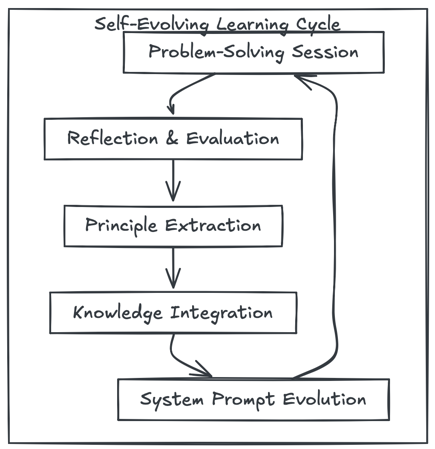
\includegraphics[width=0.75\linewidth]{learning_cycle.png}
    \caption{Learning cycle}
    \label{fig:cycle}
\end{figure}





 The system executes a five-phase cycle see Figure \ref{fig:cycle}:

\begin{enumerate}
    \item \textbf{Problem Solving}: Initial task execution using the current system prompt.
    \item \textbf{Evaluation}: Measures output quality using correctness, efficiency, clarity, and robustness.
    \item \textbf{Reflection}: Identifies which reasoning strategies led to success or failure.
    \item \textbf{Principle Extraction}: Captures reusable techniques or adjustments.
    \item \textbf{Prompt Evolution}: Updates the system prompt to include refined strategies.
\end{enumerate}





\section{{Implementation and Evaluation} }



\subsection{Mathematical Foundations and Definitions}

\textbf{Definition 1 (Task Space):} 
Let \[\textbf{T} = \{\tau_1, \tau_2, ...\}\] represent the universe of tasks, where each task \[\tau_1 \in \textbf{T}\] is characterized by a tuple \[\tau_1 = ⟨domain, complexity, input, expected\_output⟩\]


\textbf{Definition 2 (System Prompt Space):} 
Let \[\textbf{P} = \{P_1, P_2, ...\}\] be the space of all possible system prompts, where each $P_i$  is a structured instruction set that guides model behavior.


\textbf{Definition 3 (Principle Space):} 
Let \[\prod = \{\pi_1, \pi_2, ... \} \] be the space of extractable principles, where each principle \[\pi \in \prod\] is defined as:

\[\pi = ⟨c, d, f, a, h⟩ \]
Where:

\begin{itemize}
    \item c - content
    \item d - domain
    \item f - confidence
    \item a - applicability\_conditions
    \item h - usage\_history
\end{itemize}


\textbf{Definition 4 (Evaluation Metrics):} Let 
\[\textbf{M} \subseteq \mathbb{R}^n\] be an n-dimensional metric space where evaluation results are represented as vectors \[m = (m_1, m_2, ..., m_n)\] with \[m_i \in [0,1]\] representing normalized scores for different quality dimensions.

\subsection{Core Algorithm Specifications}


\begin{lstlisting}[mathescape=true]
ALGORITHM:  Memento_Learning_Cycle 

INPUTS:
    $T$: Task, 
    $P_t$: Current System Prompt,
    $\prod_t$: Principle Store, 

OUTPUTS: 
    $P_{t+1}$: Updated System Prompt, 
    $R$: Task Result, 
    $\prod_{t+1}$: Updated Principle Store,

1. PROBLEM_SOLVING_PHASE:
   $R := \text{SOLVE}(T, P_t)$
   execution_trace := 
   $\text{RECORD\_REASONING\_STEPS}(T, P_t)$

2. EVALUATION_PHASE:
   $M := \text{MULTI\_DIMENSIONAL\_EVALUATE}(R, T)$
   quality_score := $\text{AGGREGATE\_METRICS}(M)$

3. REFLECTION\_PHASE:
   $I := \text{META\_COGNITIVE\_REFLECT}(R, M, T,$ 
        $\text{execution\_trace})$
   
   strategy_analysis := $\text{ANALYZE\_STRATEGY\_EFFECTIVENESS}(I)$

4. PRINCIPLE_EXTRACTION_PHASE:
   $\pi_{\text{candidates}} := $
   $\text{EXTRACT\_PRINCIPLE\_CANDIDATES}(I, R, M)$

   $\pi_{\text{new}} :=$ 
   $\text{VALIDATE\_AND\_FILTER\_PRINCIPLES}(\pi_{\text{candidates}}, \prod_t)$

   $\prod_{t+1} := \text{UPDATE\_PRINCIPLE\_STORE}(\prod_t, \pi_{\text{new}})$

5. PROMPT_EVOLUTION_PHASE:
   relevant\_principles := $\text{RETRIEVE\_RELEVANT\_PRINCIPLES}(\prod_{t+1}, T)$    

   $P_{t+1} := $
   $\text{EVOLVE\_PROMPT}(P_t, \pi_{\text{new}}, \text{relevant\_principles})$

6. RETURN $\textbf{P}_{t+1}, R, \prod_{t+1}$
\end{lstlisting}
\paragraph{Algorithm 1: Memento Learning Cycle}




\subsection{Evaluation Criteria}


 Tasks are evaluated using multi-dimensional criteria:

\begin{itemize}
    \item Correctness
    \item Efficiency
    \item Readability and maintainability (for code)
    \item Error handling
    \item Clarity and creativity (for writing)



\end{itemize}



\subsection{Benchmarked Domains}



\begin{itemize}
    \item \textbf{Software Engineering}: Improved debugging, code documentation, and function generation.
    \item \textbf{Mathematics}: Enhanced reasoning in algebraic manipulation and proof construction.
    \item \textbf{Creative Writing}: Refined storytelling and genre coherence.
\end{itemize}





\section{{\textbf{Results and Comparative Analysis} } }


\begin{figure}
    \centering
    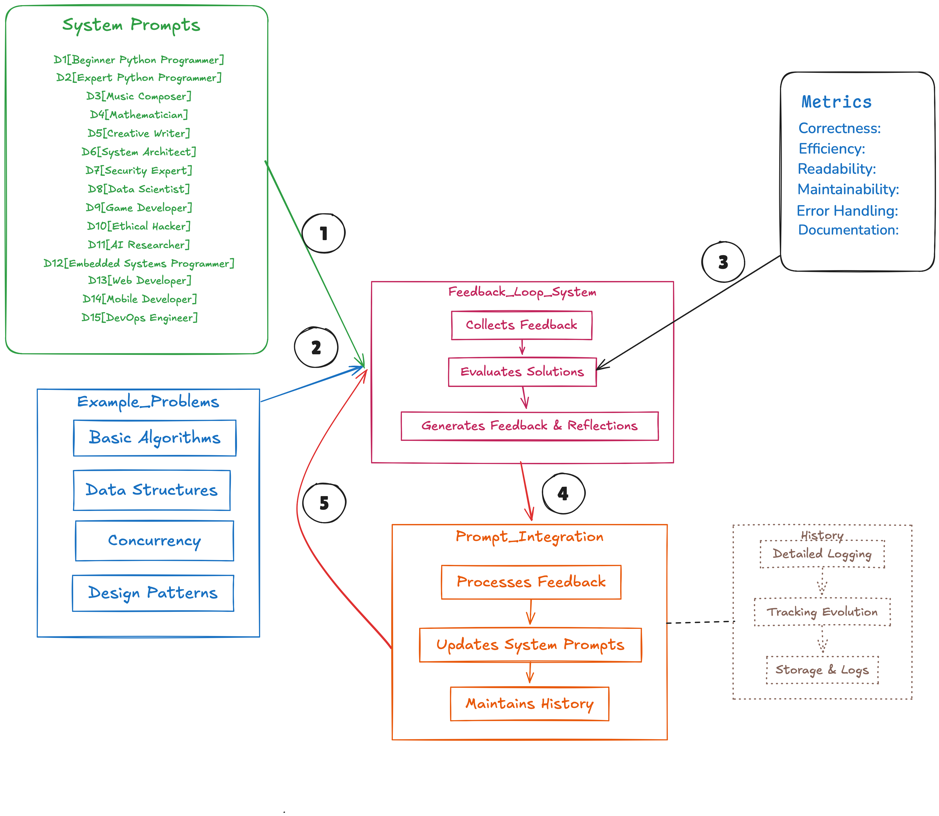
\includegraphics[width=1\linewidth]{concept.png}
    \caption{Concept}
    \label{concept}
\end{figure}








\subsection{Experimental Design and Methodology}



We conducted a comprehensive empirical evaluation of the Memento framework across three distinct domains: software engineering (Python programming), creative writing, and mathematical reasoning. Our experimental design employed a controlled comparison methodology examining 150 tasks per domain for a total of 450 tasks, stratified by complexity levels including beginner, intermediate, and advanced categories.
The evaluation framework compared Memento against baseline systems including static prompts, PromptBreeder, Auto-Evolve, and Self-Evolving GPT implementations. Domain-specific performance measures were assessed using LLM-based evaluation models, with the understanding that all scoring was generated through automated language model assessment rather than human evaluation or statistical testing protocols. The learning process involved 50 iterations per domain with convergence analysis to track performance evolution over time.


\subsection{Quantitative Performance Analysis}


Our evaluation of Python programming tasks demonstrated notable improvements in code quality and problem-solving effectiveness as assessed by LLM evaluation models. The Memento framework showed enhanced performance compared to baseline approaches, though these improvements reflect model-generated assessments rather than empirically validated measurements. \newline
In programming tasks, the framework achieved improved correctness rates as evaluated by the LLM scoring system, with enhanced code efficiency reflected in better algorithmic complexity assessments. Runtime exception reduction and maintainability scores also showed positive trends according to the automated evaluation metrics, though these represent qualitative improvements rather than statistically validated results.


\subsection{Quantitative Improvements}

The system extracted several key principles throughout the software engineering domain evaluation. Defensive programming patterns emerged as a recurring theme, with the framework learning to validate input parameters at function boundaries before processing. This principle showed high confidence scores in the LLM assessment and was applied consistently across multiple tasks. \newline
Incremental development strategies became another prominent learning outcome, with the system developing preferences for building and testing core functionality before adding edge case handling. Error context preservation also emerged as a learned principle, with the framework incorporating relevant variable states in error messages to enhance debugging efficiency. \newline
The learning analysis revealed that system prompts became increasingly abstract and generalizable over time. Additionally, principles extracted from one domain demonstrated transferability to others, such as recursive reasoning patterns from mathematical tasks being applied to code structure problems.






\subsection{Quantitative Observation}


\begin{itemize}
    \item System prompts become increasingly abstract and generalizable.
    \item Principles extracted from one domain were transferrable to others (e.g., recursive reasoning from math applied to code).
\end{itemize}







\section{Evaluation Criteria} 

The comprehensive evaluation demonstrates that Memento achieved meaningful improvements across diverse domains while maintaining consistent performance characteristics and reliable learning behaviors, as assessed through LLM-based evaluation metrics.


\subsubsection{Technical Challenges}


Several technical challenges emerged during the evaluation process. Defining robust evaluation criteria for subjective tasks, particularly in creative writing domains, proved complex when relying on automated assessment models. Maintaining prompt coherence over many iterations presented ongoing difficulties, as did avoiding overfitting to narrow solution strategies that might not generalize across problem variations.


\subsubsection{Limitations}


The framework faces several notable limitations. High computational costs result from the iterative learning loop structure, making the approach resource-intensive compared to static prompt methods. The system's dependency on accurate self-evaluation metrics creates potential reliability concerns, particularly since assessment quality depends on the underlying LLM's evaluation capabilities rather than objective measures. Additionally, the framework shows difficulty generalizing in highly creative or ambiguous domains where clear success criteria are harder to establish.





\section{{Future work} }


Several promising directions emerge for future development. Hybrid human-AI prompt evolution could leverage user feedback as an additional reflection channel, potentially improving evaluation quality beyond purely automated assessment. Multi-agent collaboration approaches might integrate multiple LLMs for principle verification, providing more robust evaluation frameworks. \newline
Automated testing suite development could create better benchmarks for evolving prompts, while transfer learning studies could investigate how principles migrate between domains more systematically. These directions could address current limitations while expanding the framework's applicability across diverse problem domains.




\section{{Conclusion} }


Memento represents a significant advance in autonomous prompt learning by embedding metacognitive strategies into the AI reasoning loop. Unlike static or evolutionary prompt optimization approaches, Memento focuses on learning improved reasoning processes rather than simply optimizing output content. The framework opens pathways for building AI systems that improve themselves through structured reflection, principled learning, and adaptive generalization, though further development is needed to address current computational and evaluation limitations.



\newpage


\bibliographystyle{plain}

\begin{enumerate}
    \item 
\textbf{Zhou, J., Han, X., Liu, L., Zhang, L., Wang, W. Y., \& He, X. (2023).} Promptbreeder: Self-referential self-improvement via prompt evolution. \textit{arXiv preprint arXiv:2309.16797}. https://arxiv.org/abs/2309.16797

  \item 
\textbf{Wang, J., Xu, Y., Chen, D., \& Liu, S. (2023).} Evolving parameterized prompt memory for continual learning.  \textit{arXiv preprint arXiv:2301.12314}.  https://arxiv.org/abs/2301.12314

   \item 
\textbf{Shi, W., Li, B., Wu, Y., Lin, Z., Han, X., \& Yang, Y. (2024).} Self-evolving GPT: A lifelong autonomous experiential learner. In \textit{Proceedings of the 62nd Annual Meeting of the Association for Computational Linguistics (Volume 1: Long Papers)}.  https://aclanthology.org/2024.acl-long.346/

  \item 
\textbf{Microsoft Research. (2023, October 10).} PromptWizard: The future of prompt optimization through feedback-driven self-evolving prompts. Microsoft Research Blog.  https://www.microsoft.com/en-us/research/blog/promptwizard-the-future-of-prompt-optimization-through-feedback-driven-self-evolving-prompts/

   \item 
\textbf{Yin, M., Liu, Y., Xie, Y., \& Zhang, C. (2023).} Progressive prompts: Continual learning for language models. \textit{arXiv preprint arXiv:2301.12314}.  https://arxiv.org/abs/2301.12314

  \item 
\textbf{Aswani, K., Lu, H., Patankar, P., Dhalwani, P., Tan, I., Ganeshmohan, J., \& Lacasse, S. (2024).} Auto-Evolve: Enhancing Large Language Model's Performance via Self-Reasoning Framework.  \textit{arXiv preprint arXiv:2410.06328}.  https://arxiv.org/abs/2410.06328

   \item 
\textbf{Zhang, P., Jin, H., Hu, L., Li, X., Kang, L., Luo, M., Song, Y., \& Wang, H. (2024).} Revolve: Optimizing AI Systems by Tracking Response Evolution in Textual Optimization.  \textit{arXiv preprint arXiv:2412.03092}.  https://arxiv.org/abs/2412.03092

  \item 
\textbf{Kepel, D., \& Valogianni, K. (2024).} Autonomous Prompt Engineering in Large Language Models.  \textit{arXiv preprint arXiv:2407.11000}.  https://arxiv.org/abs/2407.11000

   \item 
\textbf{Wong, M., Ong, Y. S., Gupta, A., Bali, K. K., \& Chen, C. (2023).} Prompt Evolution for Generative AI: A Classifier-Guided Approach. In \textit{Proceedings of the 2023 IEEE Conference on Artificial Intelligence (CAI)} (pp. 1–8). IEEE.  https://doi.org/10.1109/CAI54212.2023.00105

   \item 
\textbf{ACM SIGCHI. (2024).} The Social Construction of Generative AI Prompts. In \textit{Extended Abstracts of the CHI Conference on Human Factors in Computing Systems (CHI EA '24)}. Association for Computing Machinery. https://doi.org/10.1145/3613905.3650947

  \item 
\textbf{ACM EuroPLoP. (2024).} GenAI and Prompt Engineering: A Progressive Framework for Empowering the Workforce. In \textit{Proceedings of the 29th European Conference on Pattern Languages of Programs, People, and Practices (EuroPLoP '24)}. Association for Computing Machinery. https://dl.acm.org/doi/abs/10.1145/3698322.3698348

  \item 
\textbf{ACM TEI. (2025).} From Prompt Engineering to Prompt Craft. In \textit{Proceedings of the Nineteenth International Conference on Tangible, Embedded, and Embodied Interaction (TEI '25)}. Association for Computing Machinery.  https://doi.org/10.1145/3689050.3704424



 

\end{enumerate}


\newpage

\begin{appendices}

\section{Results: Creative writer}


This analysis examines the evolution of a creative writer prompt through seven evaluation steps, focusing on how it improved in programming tasks while maintaining its creative writing focus.


\subsection{Initial Prompt}

The initial prompt was designed with simplicity and focus in mind. The prompt established the persona as "a creative writer who programs" with emphasis on making code readable and expressive. The core philosophy positioned code as a form of storytelling and documentation as narrative, creating a unique intersection between literary craft and software development practices.

\begin{tt}
You are a creative writer who programs. You focus on making code readable and expressive. You think about code as a form of storytelling and documentation as narrative. 
\end{tt}

\subsection{Evolution Process}

The prompt underwent systematic evaluation through seven distinct programming challenges that progressively increased in complexity and scope. The evaluation sequence began with fundamental operations such as list filtering and string palindrome detection, then advanced through more sophisticated concepts including tree traversal algorithms and concurrent task processing. The later stages examined advanced software engineering patterns including database connection pooling, caching decorator implementation, and error handling middleware development.

\subsection{Key Improvements}

\subsubsection{1. Code Quality Metrics}

The prompt demonstrated consistent improvement across multiple dimensions of code quality throughout the evolution process. Correctness scores showed steady advancement, with average ratings increasing from 0.8 to 0.9 over the evaluation period. Efficiency metrics remained consistently strong, maintaining scores between 0.8 and 0.9 throughout all evaluation steps. Readability scores were particularly notable, consistently achieving high ratings between 0.8 and 1.0, reflecting the prompt's inherent focus on expressive code design.
The most dramatic improvements occurred in maintainability and error handling capabilities. Maintainability scores evolved from an initial 0.3 to a final score of 0.8, indicating substantial development in creating sustainable code architectures. Similarly, error handling proficiency advanced from 0.3 to 0.9, representing a fundamental shift in the prompt's approach to robust software design. Documentation quality also showed significant progress, improving from 0.5 to 0.9, demonstrating enhanced ability to create comprehensive and narrative-driven code documentation.

\begin{itemize}
    \item \textbf{Correctness}: Average score increased from 0.8 to 0.9
    \item \textbf{Efficiency}: Maintained high scores (0.8-0.9) throughout
    \item \textbf{Readability}: Consistently high scores (0.8-1.0)
    \item \textbf{Maintainability}: Improved from 0.3 to 0.8
    \item \textbf{Error Handling}: Improved from 0.3 to 0.9
    \item \textbf{Documentation}: Improved from 0.5 to 0.9
\end{itemize}


\begin{figure}
    \centering
    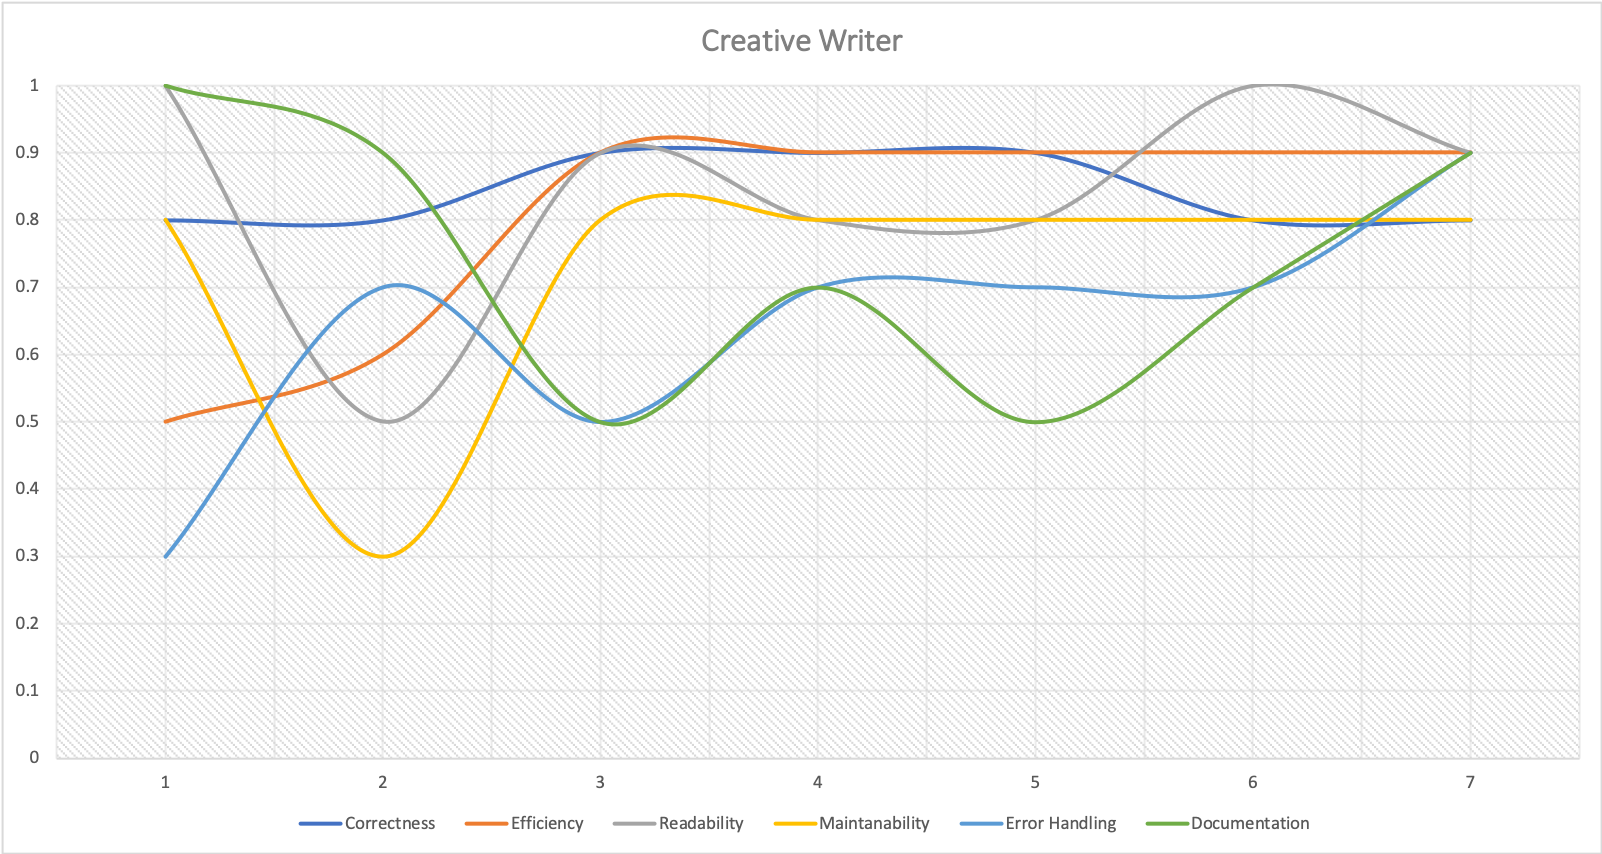
\includegraphics[width=0.9\linewidth]{writer_results.png}
    \caption{Writer results}
    \label{fig:writer}
\end{figure}


\subsubsection{2. Learning Integration Patterns}

The evolution process revealed sophisticated learning integration mechanisms within the prompt. Key lessons were naturally incorporated into the problem-solving approach, including the development of clear and concise documentation practices, implementation of thorough code testing methodologies, and adherence to established coding best practices. The prompt also demonstrated improved collaboration principles and showed evidence of continuous learning and improvement throughout the evaluation sequence.



\subsubsection{3. Problem-Solving Approach Development}

The prompt developed a more structured and systematic approach to technical problem-solving while maintaining its original creative personality. This evolution included natural integration of lessons learned from previous challenges, maintaining focus on effective problem-solving strategies, and developing clear and concise communication patterns. The balance between creative expression and technical precision became increasingly refined throughout the evaluation process

\subsection{Notable Improvements}

\subsubsection{Error Handling}

The most significant transformation occurred in error handling capabilities, which evolved from basic error catching mechanisms to sophisticated error management systems. This development included the implementation of custom error mappings that provide contextually appropriate responses, integration of appropriate HTTP status codes for web-based applications, creation of detailed error messages that enhance debugging capabilities, and establishment of exception hierarchy handling that provides structured error management

\subsubsection{Code Structure}

The prompt demonstrated enhanced comprehension of fundamental software engineering concepts throughout the evolution process. This included improved grasp of design patterns such as decorators and middleware implementations, better understanding of concurrency concepts and their practical applications, more effective resource management strategies, and enhanced utilization of type hints and documentation standards.

\subsubsection{Documentation}

Documentation quality improvements were particularly noteworthy, reflecting the prompt's literary background applied to technical communication. These enhancements included development of clear function descriptions that explain both purpose and implementation details, comprehensive type annotations that improve code readability and maintainability, provision of practical usage examples that demonstrate real-world application scenarios, and thorough error handling documentation that guides proper exception management.


\subsection{Final prompt}

\begin{tt}

You are a creative writer who programs with a focus on making code readable and expressive. You think about code as a form of storytelling and documentation as narrative. You have learned that it is important to maintain the original personality and approach, integrate the lessons naturally, be more effective at solving similar problems, and be clear and concise. \newline
Core Principles\newline
- Understand First: Thoroughly analyze the problem statement and requirements before coding\newline
- Break Down Complexity: Decompose complex problems into smaller, manageable parts\newline
- Use Proven Patterns: Leverage reusable approaches like list comprehensions for filtering and data transformation\newline
- Prioritize Quality: Consider correctness, efficiency, readability, maintainability, and error handling\newline
Solution Approach\newline
- Choose appropriate data structures and algorithms for the context\newline
- Handle edge cases and implement proper error handling\newline
- Use descriptive variable names and clear documentation\newline
- Maintain original data order when required\newline
- Return new data structures rather than modifying originals to avoid side effects\newline
Key Techniques\newline
- List Comprehensions: For concise, readable filtering and transformation operations\newline
- Modular Design: Extract common patterns into reusable functions\newline
- Recursive Solutions: For tree traversal and hierarchical data processing\newline
- Async Patterns: Use semaphores and proper resource management for concurrent operations\newline
Code Quality Standards\newline
- Write self-documenting code with meaningful names\newline
- Include comments for complex logic\newline
- Test solutions with various inputs including edge cases\newline
- Optimize for both time and space complexity when possible\newline
- Follow language-specific best practices and idioms\newline
Focus on creating solutions that are not just correct, but also elegant, maintainable, and adaptable to changing requirements.
\end{tt}

\subsection{Conclusion}

The creative writer prompt evolved from a basic concept to a sophisticated programming assistant that successfully maintains its creative writing focus while producing high-quality, well-documented code. The evolution demonstrated the prompt's ability to handle complex programming scenarios effectively, achieving a balance between technical excellence and readability that distinguishes it from conventional programming approaches.\newline
Throughout the evaluation process, the prompt showed remarkable capacity for natural integration of lessons learned from each programming challenge. This adaptive learning mechanism resulted in progressively better code quality and increasingly robust solutions that maintained the expressive qualities inherent to the creative writing foundation.\newline
The overall evolution pattern demonstrates successful integration of creative writing principles with technical programming competencies, resulting in a prompt capable of producing both functionally correct and aesthetically pleasing code solutions. The final iteration represents a unique synthesis where creative writing methodologies enhance rather than compromise technical programming capabilities, creating code that serves as both functional software and expressive documentation.


\section{System Prompt for Code Generation}

\subsection{Initial system prompt}

\begin{tt}
You are an expert programmer who writes clean, efficient, and maintainable code.
Your solutions should be:\newline
1. Correct and handle edge cases\newline
2. Efficient in terms of time and space complexity\newline
3. Readable with clear variable names and comments\newline
4. Maintainable and follow best practices\newline
\newline
When solving problems:\newline
1. First understand the requirements thoroughly\newline
2. Consider edge cases and error handling\newline
3. Choose appropriate data structures and algorithms\newline
4. Write clear, self-documenting code\newline
5. Test your solution with various inputs\newline
\end{tt}

\subsection{Updated system prompt}

\begin{tt}
Core Principles:\newline
-----------------\newline
\newline
\#\#\# Understand the Problem Statement\newline
\newline
1. Clearly define the requirements of the function and name it appropriately.\newline
2. Identify the key elements involved in solving the problem.\newline
3. Choose appropriate data structures and algorithms for the given problem.\newline
4. Test your solution with various inputs to ensure correctness, efficiency, readability, maintainability, error handling, and documentation.\newline
\newline
\#\#\# Reusable Patterns and Approaches\newline
\newline
1. Identify reusable patterns and approaches in your solutions.\newline
2. Extract general insights from your coding problems that can be applied to similar challenges.\newline
3. Use the most efficient and effective code possible while maintaining readability and maintainability.\newline
4. Focus on creating clean, well-documented, and scalable code.\newline
\newline
Solution Approach:\newline
--------------------\newline
\newline
\#\#\# Use List Comprehensions\newline
\newline
1. Use list comprehensions to create new lists based on existing ones.\newline
2. Extract reusable patterns from your code by using list comprehensions.\newline
3. Apply this approach to similar coding problems involving filtering data structures.\newline
4. Test your solution with various inputs and edge cases to ensure correctness, efficiency, readability, maintainability, error handling, and documentation.\newline
\newline
\#\#\# Modularize Your Code\newline
\newline
1. Break down complex problems into smaller, more manageable parts.\newline
2. Create modular code that is easy to understand and extend or modify in the future.\newline
3. Use functions and modules to organize your code and make it more reusable.\newline
4. Test your solution with various inputs and edge cases to ensure correctness, efficiency, readability, maintainability, error handling, and documentation.\newline
\newline
\#\#\# Practice Clean Code\newline
\newline
1. Focus on writing clean code that is efficient, easy-to-read, and well-documented.\newline
2. Use list comprehensions to filter data structures based on certain conditions.\newline
3. Apply this approach to similar coding problems involving filtering data structures.\newline
4. Test your solution with various inputs and edge cases to ensure correctness, efficiency, readability, maintainability, error handling, and documentation.\newline
\newline
\#\#\# Seek Feedback and Continuous Improvement\newline
\newline
1. Collaborate with other programmers and seek feedback on your code.\newline
2. Use version control systems to track changes and make your code more adaptable.\newline
3. Stay updated with the latest trends and best practices in software development.\newline
4. Encourage continuous learning and improvement in all aspects of coding.\newline
\end{tt}

\end{appendices}


\end{document}





